%Template pembuatan proposal skripsi.
\documentclass{jtetiproposalskripsi}

%-----------------------------------------------------------------
%Disini awal masukan untuk data proposal skripsi
%-----------------------------------------------------------------
\titleind{SISTEM INFORMASI AKADEMIK SEKOLAH PADA SMA MUHAMMADIYAH 3 JEMBER}

\fullname{YULIO RIZKI}

\idnum{1200631027}

\approvaldate{13 November 2015}

\degree{Sarjana Teknik Elektro}

\yearsubmit{2015}

\program{Manajemen Informatika}

\headprogram{Sarjiya, S.T., M.T., Ph.D.}

\dept{Teknik Elektro dan Teknologi Informasi}

\firstsupervisor{Triawan Adi Cahyanto,M.Kom}
\firstnip{ 12 03 719}

\secondsupervisor{Bagus Setya Rintyarna,S.T,M.Kom}
\secondnip{09 03 521}


%-----------------------------------------------------------------
%Disini akhir masukan untuk data proposal skripsi
%-----------------------------------------------------------------

\begin{document}

\cover

\approvalpage

%-----------------------------------------------------------------
%Disini akhir masukan untuk muka skripsi
%-----------------------------------------------------------------

%-----------------------------------------------------------------
%Disini awal masukan Intisari
%-----------------------------------------------------------------
\begin{abstractind}
Aplikasi sistem informasi akademik memudahkan pengguna untuk melakukan kegiatan administratif akademik. Fungsinya adalah untuk membantu seluruh komponen sekolah dalam pengelolaan data nilai siswa, mata pelajaran , data pengajar (guru) serta administrasi sekolah yang sifatnya masih manual untuk dikerjakan dengan bantuan Software agar mampu mengefektifkan waktu dan menekan biaya operasional. Masalah keterbatasan fleksibilitas akses sistem informasi akadeik yang mengharuskan pengguna terhubug dengan internet secara statis menyebabkan perlu  dirancang suatu aplikasi sistem informasi akademik sekolah yang mampu memenuhi kebutuhan fleksibilitas dari para user untuk dapat melakukan akses dengan lebih mudah dan cepat.\\

Dengan menggunakan perangkat lunak PHP dan MySQL  sebagai media untuk mengembangkan sistem informasi akademik sekolah berbasis web ini bertujuan untuk mengembangkan sistem akademik sekolahdi SMAMuhammadiyah 3 jember \\

Penelitian ini bertujuan untuk  merancang sistem informasi akademik  berbasis web, yang dapat diakses melalui website sekolah tersebut untukmemudahkan akses yang lebih fleksibel



\bigskip
\textbf{Kata kunci} : website, Sistem Informasi Akademik, PHP.
\end{abstractind}
%-----------------------------------------------------------------
%Disini akhir masukan Intisari
%-----------------------------------------------------------------

\tableofcontents
\addcontentsline{toc}{chapter}{DAFTAR ISI}
\selectlanguage{bahasa}\clearpage\pagenumbering{arabic}\setcounter{page}{1}

%-----------------------------------------------------------------
%Disini awal masukan untuk Bab
%-----------------------------------------------------------------
\chapter{LATAR BELAKANG}

\section{Latar Belakang Masalah}
Perkembangan ilmu pengetahuan dan teknologi khususnya teknologi informasi yang semakin pesat di dalam semua bidang.Teknologi Informasi merupakan alat untuk mempermudah ,dan  mempercepat pekerjaan. Selain itu teknologi juga memungkinkan sebuah infomasi dapat diakses dalam waktu kapanpun.\\

SMA Muhammadiyah 3 Jember adalah sebuah sekolah menengah keatas yang pada awalnya memiliki puluhan siswa saja, namun seiring berjalannya waktu , jumlah siswa dari tahun ketahun selalu mengalami peningkatan, tenaga pengajar dan staff karyawan.\\

Dengan banyaknya jumlah siswa dari tahun ke tahun ini 	membuat para guru mengalami kesulitan dalam mengolah nilai siswa. Ada beberapa kendala lain yang dihadapi oleh para guru ,dan siswa mengakses informasi sekolah tersebut
Kalau diperhatikan dalam kemajuan yang telah dicapai oleh institusi pendidikan tersebut ,maka terlihat dengang jelas bahwa permasalahannya adalah terletak pada sebuah data dan teknologi informasi yang akurat. Penerapan suatu sistem data dan informasi sebenarnya tidak terlepas dari penggunaan alat elektronik yang dapat mempermudah proses penanganan sistem informasi.\\

Setelah meninjau permasalahan pada penggunaan data dan informasi yang akurat , maka penulis mempunyai keingan untuk membuat sebuah sistem informasi berbasi web pada SMA Muhammadiyah 3 Jember . Oleh karena itu , pada kesempatan ini penulis mengkhususkan pembuatan aplikasi sistem informasi akdemik sekolah berbasis web. Pembuatan sistem informasi ini didasarkan atas keinginan penulis menyidiakan informasi tenang akademik siswa dan memudahkan para guru di sekolah tersebut untuk memasukkan nilai-nilai dari para siswa. Dengan sebuah sistem informasi berbasis web ini para guru , pegawai sekolahtersebut akan dengan mudah mengakses dan mengetahui segala sesuatu mengenai akademik para siswa tersebut dengan mudah tanpa harus datang ke bagian tata usaha terlebih dahulu dan tidak  membutuhkan waktu yang banyak.
\section{Rumusan Masalah}
Berdasarkan Urain dari latar belakang permasalahan di atas, maka masalah yang  akan dibahas adalah sebagai berikut :
\begin{itemize}


\item[1.]	Apakah sistem informasi yang dibangun sudah baik, sehingga pihak SMA Muhammadiyah 3 Jember sendiri dapat berinteraksi di web tersebut?
\item[2.]	Informasi apa saja  yang disediakan dalam web sekolah tersebut, sehingga para guru , pegawai , dan siswa  mendapatkan informasi yang efektif dan akurat?
\item[3.] Apakah sistem informasi yang dibangun berguna bagi pihak sekolah sendiri?
\end{itemize}

\section{Batasan Masalah}
Batasan masalah dalam pembuatan Program ini diantaranya :
\begin{itemize}


\item[1.]	Penggunaan aplikasi ini adalah para guru , siswa dan staff karyawan di SMA Muhammadiyah 3 Jember
\item[2.]	System hanya menangani dan membahas tentang pengolahan data nilai siswa, mata pelajaran dan data pengajar.
\item[3.] System ini merupakan sistem basis data yang dibangun menggunakan php dan MySQL sebagai databasenya 
\end{itemize}

\section{Maksud dan Tujuan}
Maksud dan tujuan pembahasan ini diantaranya :
\begin{itemize}

\item[1.]Membangun Sistem informasi Akademik sekolah yang efektif dan efisien berbasis web
\item[2.]Untuk memberikan informasi yang cepat dan akurat pada siswa
\item[3.]Mendukung rencana pemanfaatan fasilitas yang tersedia dengan membuat sistem informasi akdemik sekolah
\end{itemize}




\section{Manfaat Program}
Sistem Informasi Akademik Sekolah mempunyai banyak manfaat bagi semua komponen sekolah . Selain mempermudah dan melihat proses administrasi pendidikan , Sistem Inforamsi Akademik Sekolah juga meningkatkan transparansi informasi kepada publik.
Adapun manfaat dari Sistem Informasi Akademik Sekolah adalah sebagai berikut :
\begin{itemize}


\item[1.] Mempermudah pendataan guru , siswa , mata pelajaran , nilai dan kegiatan akademik sekolah
\item[2.]	Mempermudah dan mempercepat proses pencarian informasi akademik sekolah
\item[3.]	Meningkatkan efisiensi terutama karena berkurangnya  dokumen yang harus dicetak 
\item[4.]	Meningkatkan transparansi informasi akademik sekolah
\item[5.]	Meningkatkan Prestasi sekolah
\end{itemize}

%-------------------------------------------------------------------------------
\chapter{TINJAUAN PUSTAKA DAN DASAR TEORI}                

\section{Landasan Teori}
\subsection{Sistem Informasi}
Menurut Jhon F. Nash (1995:8) yang diterjemahkan oleh LaMidjan dan Azhar Susanto, menyatakan bahwa sistem informasi adalahkombinasi dari manusia, fasilitas atau alat teknologi, media, prosedur dan pengendalian yang bermaksud menata jaringan komunikasi yang penting, proses atas transaksi-transaksi tertentu dan rutin, membantu manajemendan pemakai intern dan ekstern dan menyediakan dasar pengambilankeputusan yang tepat.Sedangkan menurut Henry Lucas (1988:35) yang diterjemahkanoleh Jugianto H.M, menyatakan bahwa sistem informasi adalah suatukegiatan dari prosedur-prosedur yang diorganisasikan, bilamanadieksekusi akan menyediakan informasi untuk mendukung pengambilankeputusan dan pengendalian di dalam organisasi.Dari kedua pengertian sistem informasi diatas, maka dapatdisimpulkan bahwa sistem informasi menyediakan informasi untukmembantu pengambilan keputusan manajemen, operasi perusahaan darihari ke hari dan informasi yang layak untuk pihak luar perusahaan.(Jogiyanto,2005)


\subsection{Akademik}
Sistem informasi akademik adalah perangkat lunak yangdigunakan untuk menyajikan informasi dan menata administrasi yang berhubungan dengan kegiatan akademik. Dengan penggunaan perangkat lunak seperti ini diharapkan kegiatan administasi akademik dapatdikelola dengan baik dan informasi yang diperlukan dapat diperolehdengan mudah dan cepat (Jogianto,2005).Sistem informasi dapat didefinisikan sebagai suatu sistem dalamsuatu organisasi yang merupakan kombinasi dari orang-orang, fasilitas,teknologi, media prosedur-prosedur dan pengendalian yang ditunjukkanuntuk mendapatkan jalur komunikasi penting, memproses tipe transaksirutin tertentu, memberi sinyal kepada manajemen dan yang lainnyaterhadap kejadian-kejadian internal dan ekternal yang penting danmenyediakan suatu dasar informasi untuk pengambilan keputusan.

\subsection{Web}

Web merupakan sistem dengan standar yang diterima secarauniversal untuk menyimpan, menelusuri, memformat dan menyimpaninformasi melalui arsitektur Klien atau server. Web bisa menerima semua jenis informasi digital, termasik teks, hipermedia, grafis dan suara. Webdidasari oleh hiperteks standar yang disebut  HyperText Markup Language (HTML), yang memformat dokumen dan memadukan linkhiperteks dinamis ke dokumen-dokumen lainnya yang disimpan di dalamkomputer yang sama atau berbeda. (Turban,dkk. 2006). 

\subsection{Database}
Database (basis data) adalah sekumpulan data yang digambarkan sebagai aktivitas dari satu atau lebih organisasi yang  berelasi. Keuntungan menggunakan database dalam mengelola data adalah kebebasan data dan akses yang efisien, administrasi keseragaman data, bersamaan dan perbaikan dari terjadinya tabrakkan proses serentak. (Kristanto, 2003).
 Database merupakan komponen terpenting dalam  pembangunan sistem informasi karena menjadi tempat untuk menampung dan mengorganisasikan seluruh data yang ada dalam sistem sehingga dapat dieksplorasi untuk menyusun informasi-informasi dalam berbagai bentuk.
 Database merupakan himpunan kelompok data yang saling berkaitan. Data tersebut diorganisasikan sedemikian rupa agar tidak terjadi duplikasi yang tidak perlu sehingga dapat diolah atau dieksplorasi secara cepat dan mudah untuk menghasilkan informasi. Sistem database terus dikembangkan oleh para ahli agar dapat diperoleh cara pengorganisasian data yang efisien dan efektif.
 
Adapun penerapan sistem Database ini antara lain untuk  pembangunan sistem informasi, persediaan barang, kepegawaian, akuntansi, pemasaran, produksi, reservasi, layanan pelanggan yang digunakan dalam perusahaan retail, perbankan, perhotelan dan  pariwisata, rumah sakit, institusi pendidikan, dan sebagainya. Adapun komponen dari database adalah :
\begin{itemize}


\item[a.] Record adalah kumpulan elemen-elemen yang saling berkaitan menginformasikan tentang suatu entity secara lengkap. Satu record mewakili satu data atau informasi tentang seseorang 
 \item[b.] Field merupakan bagian dari data. setiap file selalu terdapat kunci dari file berupa satu field atau satu set field yang dapat mewakili record. 
\item[c.] Type merupakan jenis data yang berfungsi untuk memberikan type data dari field field yang ada, misalnya D (date) jika type field berjenis tanggal dan lain-lain.
 \item[d.] Size adalah ukuran yang digunakan untuk memberikan besarnya field atau jumlah karakter dari field-field yang ada. 
\item[e.] Key merupakan kunci yang dugunakan untuk memberikan jenis kunci dalam suatu file (Madcoms, 2005).
\end{itemize}
\section{PHP}
Hypertex Preprocessor(PHP) adalah skrip yang berjalan dalam
 server  side yang di tambahkan dalam HTML. PHP itu sendiri merupakan singkatan dariPersonal Home Page Tools. Tugas akhir  ini akan membuat suatu aplikasi dapat di integrasikan kedalam HTML sehingga suatu halaman HTML tidak lagi bersifat statis, namun menjadi besifat dinamis. Sifat server side ini membuat pengerjaaan skrip tersebut dikerjakan di server sedangkan yang dikirimkan kepada browser adalah hasil proses dari skrip tersebut yang sudah berbentuk HTML.

Sementara itu, jaringan WiFi sebagai jaringan lokal nirkabel yang digunakan untuk komunikasi data dalam suatu area lokal dan sudah tersebar di berbagai tempat. Lokal yang dimaksud disini adalah area yang tidak terlalu luas yaitu dengan radius sekitar 20m atau dalam sebuah gedung. Untuk membangun jaringan lokal menggunakan WiFi, perangkat utama yang digunakan adalah Access Point (AP). AP adalah piranti yang akan menjadi koordinator dalam jaringan lokal jika diinginkan topologi bintang (star) seperti diilustrasikan pada Gambar \ref{star}.
\section{MySQL}
MySQL adalah sebuah perangkat lunak sistem manajemen basis data SQL (bahasa Inggris: database management system) atau DBMS yang multithread, multi-user, dengan sekitar 6 juta instalasi di seluruh dunia. MySQL AB membuat MySQL tersedia sebagai perangkat lunak gratis dibawah lisensi GNU General Public License (GPL), tetapi mereka juga menjual dibawah lisensi komersial untuk kasus-kasus dimana penggunaannya tidak cocok dengan penggunaan GPL.\\
MySQL adalah sebuah implementasi dari sistem manajemen basisdata relasional (RDBMS) yang didistribusikan secara gratis dibawah lisensi GPL (General Public License). Setiap pengguna dapat secara bebas menggunakan MySQL, namun dengan batasan perangkat lunak tersebut tidak boleh dijadikan produk turunan yang bersifat komersial. MySQL sebenarnya merupakan turunan salah satu konsep utama dalam basisdata yang telah ada sebelumnya; SQL (Structured Query Language). SQL adalah sebuah konsep pengoperasian basisdata, terutama untuk pemilihan atau seleksi dan pemasukan data, yang memungkinkan pengoperasian data dikerjakan dengan mudah secara otomatis.

Kehandalan suatu sistem basisdata (DBMS) dapat diketahui dari cara kerja pengoptimasi-nya dalam melakukan proses perintah-perintah SQL yang dibuat oleh pengguna maupun program-program aplikasi yang memanfaatkannya. Sebagai peladen basis data, MySQL mendukung operasi basisdata transaksional maupun operasi basisdata non-transaksional. Pada modus operasi non-transaksional, MySQL dapat dikatakan unggul dalam hal unjuk kerja dibandingkan perangkat lunak peladen basisdata kompetitor lainnya. Namun pada modus non-transaksional tidak ada jaminan atas reliabilitas terhadap data yang tersimpan, karenanya modus non-transaksional hanya cocok untuk jenis aplikasi yang tidak membutuhkan reliabilitas data seperti aplikasi blogging berbasis web (wordpress), CMS, dan sejenisnya. Untuk kebutuhan sistem yang ditujukan untuk bisnis sangat disarankan untuk menggunakan modus basisdata transaksional, hanya saja sebagai konsekuensinya unjuk kerja MySQL pada modus transaksional tidak secepat unjuk kerja pada modus non-transaksional.
\section{Analisis sistem}
Bagan alir sistem (system flowchart) berfungsi untuk memodelkan masukan, keluaran , proses maupun transaksi dengan menggunakan simbol - simbol tertentu. Pembuatan sistem flowchart harus memudahkan bagi pemakai dalam memahami alur dari system atau transaksi.(Kristanto Andri.2008) 





%-------------------------------------------------------------------------------
\chapter{METODOLOGI}

\section{Metode Pengumpulan Data}
Untuk  memperoleh  data  yang  tepat  dan  akurat  guna  kesempurnaan  sistem yang akan dibuat, digunakan beberapa metode pengumpulan data. Metode-metode tersebut antara lain:


\begin{itemize}
\item[1.]Metode observasi

Metode ini diterapkan dengan mendatangi obyek  penelitian  secara langsung.  Melihat  langsung  proses  akademis  yang  dilakukan  sehingga diketahui  secara  detail  seluruh  aktifitas  instansi  yang  diteliti.  Pelaksanaan observasi  dilakukan  beberapa  kali  untuk  memperbaiki  dokumentasi  sistem. Tujuan  observasi  untuk  mendapatkan  data  yang  benar  dengan  pengamatan secara langsung ke SMA Muhammadiyah 3 Jember.
\item[2.]Metode Wawancara

Mengumpulkan data dengan melakukan wawancara dengan sumber yang bersangkutan  secara  langsung  untuk  mengumpulkan  data-data  dengan mengajukan  sejumlah  pertanyaan  yang  berkaitan  dengan  penelitian  secara lisan.  Metode wawancara  dilakukan  kebagian  tata  usaha,   yaitu  waur 
kesiswaan,  waur kurikulum dan bagian pembayaran SPP. Metode wawancara dilakukan  hanya  1  sampai  2  kali  untuk  memperjelas  materi  wawancara. Dengan langkah ini diharapkan diperoleh  keterangan tentang proses akademis 
dan pembayaran SPP di SMA Muhammadiyah 3 Jember.
\item[3.]Metode Pustaka

Dengan  cara  mengumpulkan  data  dengan  mencari  informasi  yang dibutuhkan  untuk  dapat  menyelesaikan  tugas  akhir  yaitu  dengan  membaca buku-buku dan internet yang berkaitan dengan hal-hal sistem informasi.
\end{itemize}

\section{Langkah Penyelesaian Masalah}
\begin{itemize}
\item[1.]Analisa Sistem

Analisa ini meliputi analisa sistem yang digunakan di SMA Muhammadiyah 3 Jember dan analisa kebutuhan perangkat lunak yang akan dibangun.
\item[2.]Perancangan 

Pada  tahap  ini  dibuat  aliran  informasi,  struktur  aliran  data,  spesifikasi proses, dan perancangan aplikasi.
\item[3.]Implementasi Awal

Aplikasi  akan  diimplementasikan  ke  dalam  bentuk  program  berdasarkan hasil  analisa  dan  perancangan  yang  telah  diperoleh  dari  tahap  sebelumnya.Dalam  pengimplementasian  awal  ini  menggunakan  beberapa  hardware  dan software  sebagai berikut:
\item[1.]Seperangkat komputer dengan spesifikasi :

\item[a.]Processor Intel Dual Core
\item[b.]RAM DDR3 2 GB
\item[c.]Harddisk 500 MB
\item[d.]DVD RW 

\item[2.]Sofware (Perangkat Lunak ) yang digunakan :
\item[a.]Microsoft Windows 7
\item[b.]Latex 
\item[c.]MySQL
\item[d.]PHP
\item[e.]Dan software Pendukung lainnya

\end{itemize}

\newpage

\section{Jadwal Kegiatan}
Penelitian direncanakan akan dilaksanakan selama enam bulan. Rincian rencana jadwal penelitian dicantumkan dalam tabel berikut.

\begin{figure}[h]
\centering 
 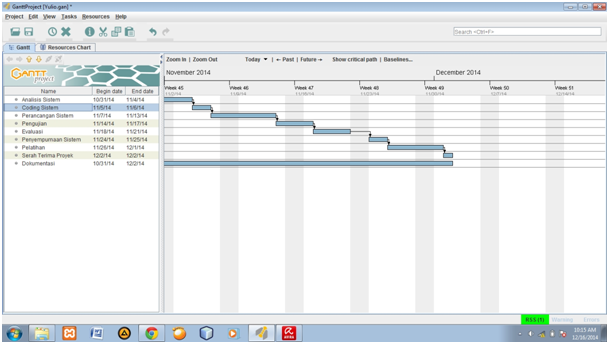
\includegraphics[width=1\textwidth]{gambar/buxxx.png}  
 \caption{Jadwal Penelitian}
\end{figure}
 
%-----------------------------------------------------------------
%Disini akhir masukan Bab
%-----------------------------------------------------------------

%-----------------------------------------------------------------
%Disini awal masukan untuk Daftar Pustaka
%-----------------------------------------------------------------
%%\nocite{Abel2010,Guerbas201350}
%%\bibliography{research-plan}
%%\bibliographystyle{plainnat}
\begin{thebibliography}{9}

\bibitem[satu(2013)]{satu01}
Fathansyah,. 2002. Basis Data. . Bandung :  Informatika.

\bibitem[dua(2013)]{dua02}
Kendall,  Kendall.  2003.  Analisa  dan  Perancangan  Sistem.  Jakarta  :   PT 
Prenhalindo.

\bibitem[tiga(2013)]{tiga03}
Arbie. 2004. Manajemen Database dengan Mysql. Yogyakarta : Andi.

\bibitem[empat(2013)]{empat04}
Sunarfrihantono, Bimo. 2002.  PHP dan MYSQL untuk WEB. Yogyakarta : Andi 
Yogyakarta.

\bibitem [lima (2013)] {lima05}
Abdul Kadir,  Pengenalan Sistem Informasi, Yogyakarta : Andi Offset 2002.

\end{thebibliography}
\addcontentsline{toc}{chapter}{DAFTAR PUSTAKA}
%-----------------------------------------------------------------
%Disini akhir masukan Daftar Pustaka
%-----------------------------------------------------------------

\end{document}